\chapter{The Transformer: A Walkthrough}\index{transformer!walkthrough}\index{architecture!transformer}

\begin{figure}[h]
\begin{center}
    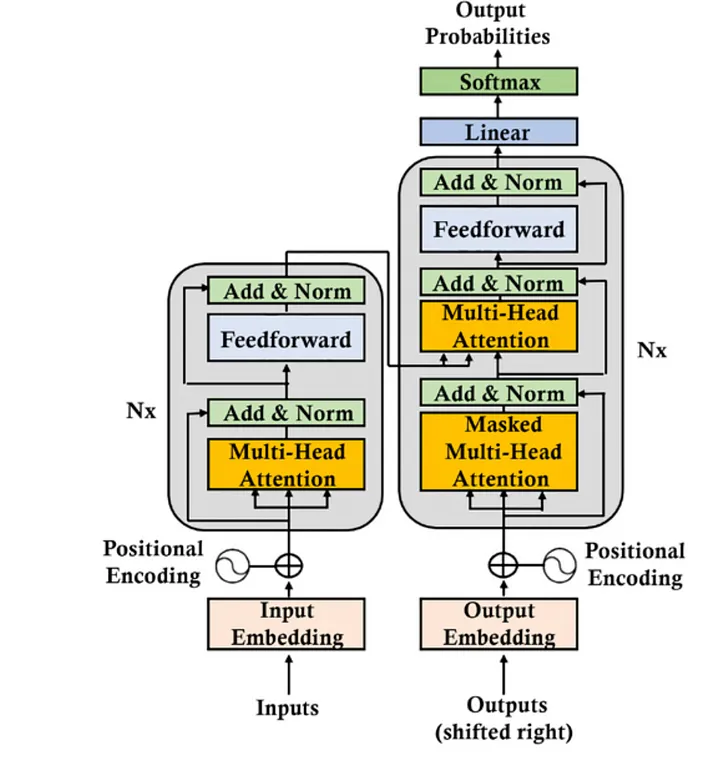
\includegraphics[width=0.8\textwidth]{images/transformer_arch.png}
    \captionof{figure}{The Transformer Architecture}
    \end{center}
\end{figure}

\section{Introduction}
\noindent
Having explored the individual components of the Transformer in previous chapters, we now examine how these elements work together to process sequences effectively. The architecture's power comes not just from its individual innovations, but from their careful integration into a cohesive system\index{transformer!system integration}.

\section{Information Flow in the Transformer}\index{transformer!information flow}
\noindent
The Transformer processes information through a carefully orchestrated sequence of operations\index{sequence processing}. The journey begins with input processing\index{input processing}, where raw text is first tokenized into discrete indices\index{tokenization}, then mapped to dense vectors through token embeddings\index{token embeddings}. These embeddings are augmented with positional encodings\index{positional encodings} (discussed in Section~\ref{sec:positional_encodings}) to preserve sequence order information\index{sequence order}, since the model processes all tokens in parallel\index{parallel processing}.

The encoder\index{encoder} then processes these enriched representations through multiple parallel blocks\index{encoder blocks}. Within each block, self-attention mechanisms\index{self-attention} (Section~\ref{sec:self_attention}) enable each token to directly interact with every other token in the sequence\index{token interaction}. Multi-head attention\index{multi-head attention} (Section~\ref{sec:multi_head_attention}) allows the model to capture different types of relationships simultaneously\index{relationship capture}, while position-wise feed-forward networks\index{feed-forward networks} transform each token's representation independently.

The decoder\index{decoder} completes the processing pipeline by generating output tokens one at a time\index{token generation}. It employs masked self-attention\index{masked self-attention} to prevent looking at future tokens during generation\index{future masking}, maintaining the causal nature of the prediction task\index{causality}. Cross-attention mechanisms\index{cross-attention} connect the decoder to the encoder's outputs\index{encoder-decoder connection}, allowing the model to draw relevant information from the input sequence while generating each new token.

\section{Architectural Synergies}\index{architectural synergies}
\noindent
The Transformer's effectiveness stems from how its components complement each other\index{component interaction}. Self-attention and positional encodings work in concert\index{attention-position synergy}, with attention providing content-based interactions while positional information maintains awareness of sequence structure\index{sequence structure}. Together, they capture both semantic relationships\index{semantic relationships} and structural patterns\index{structural patterns} in the input.

Multi-head attention and feed-forward networks form another powerful partnership\index{attention-FFN synergy}. While attention heads capture diverse relationships between tokens\index{token relationships}, the FFN layers add crucial non-linearity\index{non-linearity} and position-specific processing\index{position-specific processing}. This combination enables both rich token interactions and sophisticated feature transformations\index{feature transformation}.

The architecture's deep structure\index{deep structure} is made possible by residual connections\index{residual connections} and layer normalization\index{layer normalization} working in tandem. Residual connections preserve access to low-level features\index{feature preservation} throughout the network, while layer normalization ensures stable activation distributions\index{activation stability}. This synergy enables the reliable training of deep models that can capture hierarchical patterns in language\index{hierarchical patterns}.

\section{The Complete Pipeline}\index{transformer!pipeline}
\noindent
The full processing pipeline begins with input embedding and positioning\index{input embedding}, where discrete tokens are mapped into a continuous vector space\index{vector space} and enriched with positional information. This representation enables the parallel processing that gives the Transformer its computational efficiency\index{computational efficiency}.

The encoder stack\index{encoder stack} then builds rich contextual representations\index{contextual representations} by repeatedly applying self-attention and feed-forward transformations. Each layer in the stack captures increasingly abstract relationships\index{abstract relationships}, while maintaining the original sequence length and bidirectional context\index{bidirectional context}.

In the decoder stack\index{decoder stack}, auto-regressive generation\index{auto-regressive generation} proceeds one token at a time, with each prediction building upon previous outputs while drawing relevant information from the encoder's representations through cross-attention mechanisms. The decoder maintains causality through masked attention\index{masked attention}, ensuring predictions are based only on previously generated tokens\index{token prediction}.

Finally, the output projection layer\index{output projection} maps the decoder's representations back to the vocabulary space\index{vocabulary space}, enabling token prediction while maintaining a proper probabilistic interpretation\index{probabilistic interpretation} of the model's outputs.

\section{Design Philosophy}\index{transformer!design philosophy}
\noindent
The Transformer's design reflects several key principles that revolutionized sequence processing\index{sequence processing principles}. At its core, the architecture replaces sequential processing with parallel attention mechanisms\index{parallel attention}, enabling efficient training and inference\index{efficient training}. It provides direct access between tokens\index{direct token access}, eliminating the need for information to flow through intermediate states as in RNNs\index{RNN comparison}.

The design emphasizes stable training\index{stable training} through careful use of normalization and residual connections, allowing the construction of deep networks that can capture complex language patterns\index{language patterns}. The separation of encoding and decoding functions provides modularity\index{architectural modularity}, enabling flexible adaptation to various tasks and architectures.

For detailed mathematical formulations of these components, refer to Section~\ref{sec:transformer_notation} in the encoder block chapter.

\section{Impact on Modern Architectures}\index{transformer!modern impact}
\noindent
The Transformer architecture has spawned numerous variants\index{transformer variants} that adapt its core principles to different tasks and constraints. Encoder-only models\index{encoder-only models} like BERT\index{BERT} focus on bidirectional understanding, making them particularly suited for tasks requiring deep analysis of input text. These models excel at classification\index{classification tasks}, understanding, and analysis tasks where bidirectional context is crucial.

Decoder-only models\index{decoder-only models}, exemplified by GPT\index{GPT}, emphasize autoregressive generation\index{autoregressive generation}. By simplifying the architecture to focus on the generative aspect, these models have proven especially effective for large-scale training\index{large-scale training} and text generation tasks\index{text generation}. Their streamlined design has enabled scaling to unprecedented model sizes\index{model scaling}.

Hybrid approaches\index{hybrid approaches} have emerged that combine Transformer elements with other architectural innovations\index{architectural innovations}. These variants often optimize for specific applications\index{application-specific optimization}, demonstrating the flexibility and adaptability of the core Transformer principles\index{transformer principles}. The success of these adaptations highlights the fundamental soundness of the original design choices\index{design choices}.

\section{Training}
The Transformer is trained using a teacher-forcing method, where the ground truth output sequence (shifted one position to the right) is fed as input to the decoder. The loss function is typically cross-entropy between the predicted output distribution and the true output word.

\section{Summary}

The Transformer architecture has had a profound impact on NLP and other fields. Its ability to model long-range dependencies and its parallelizable nature have made it a powerful tool for various sequence-to-sequence tasks. This chapter provided a detailed overview of the Transformer's components and their functions. While this is a complex model, understanding its inner workings is crucial for anyone working with state-of-the-art NLP and sequence modeling techniques. Future research continues to build upon this foundation, exploring new attention mechanisms, scaling laws, and applications beyond language.
